% !TEX root = ../OT4ML.tex

\chapter{Wasserstein Space}
\index{Wasserstein!space}% strictindex
\index{Wasserstein!distance}% strictindex
\label{sec-wasserstein-space}

The preceding chapter introduced couplings as a convex relaxation of transport maps and established the Kantorovich problem as a well-posed optimization principle. When the ground cost is a power of a metric, its optimal value also equips probability measures with a metric geometry. This chapter develops the resulting Wasserstein space, from gluing and displacement geodesics to topology, stable maps on measures and distributional robustness.

%%%%%%%%%%%%%%%%%%%%%%%%%%%%%%%%%%%%%%%%%%%%%%%%%%%%%%%%%%%%%%%%%%%%%%%%%%%
\section{Wasserstein Distances}
\label{sec-wasserstein-distances}
\index{Wasserstein!distance}% strictindex


This section proves that OT costs are genuine distances when the ground cost comes from a metric. It also constructs displacement geodesics and explains how Kantorovich transport relaxes the directed Monge formulation.
\index{ground cost}% strictindex
\index{Dirac mass}% strictindex
\index{total variation}% strictindex

%%%%
\paragraph{OT defines a distance.}
\index{Wasserstein!distance}% strictindex


An important feature of OT is that it defines a distance between histograms and probability measures as soon as the cost matrix satisfies certain suitable properties. Indeed, OT can be understood as a canonical way to lift a ground distance between points to a distance between histograms or measures.
\index{histogram}% strictindex
\index{cost!matrix}% strictindex
\index{probability measure}% strictindex
%
The proof of this result relies on a ``gluing lemma'', which we first prove in the discrete case.
\index{gluing lemma}% strictindex

\begin{lem}[Discrete gluing lemma]\label{lem-gluing-discr}
	Given $(\a,\b,\VectMode{c}) \in \simplex_n \times \simplex_p \times \simplex_m$,
	let $\P \in \CouplingsD(\a,\b)$ and $\Q \in \CouplingsD(\b,\VectMode{c})$. Then there exists a nonnegative three-way array $\S \in \RR_+^{n \times p \times m}$
	such that its two-way marginals satisfy
	\eq{
		\sum_{k} \S_{i,j,k} = \P_{i,j}
		\qandq
		\sum_{i} \S_{i,j,k} = \Q_{j,k}.
	}
	Consequently the marginal between the first and third variables,
	\[
		\R_{i,k}\eqdef\sum_j \S_{i,j,k},
	\]
	belongs to $\CouplingsD(\a,\VectMode{c})$. For the canonical construction below, this glued coupling is the twisted matrix product
	\[
		\R=\P\diag(1/\b)\Q,
		\qquad
		\R_{i,k}=\sum_{j:\b_j>0}\frac{\P_{i,j}\Q_{j,k}}{\b_j}.
	\]
	In the matrix notation, $1/\b_j$ is understood as $0$ when $\b_j=0$.
\index{gluing lemma}% strictindex
\end{lem}
\begin{proof}
	\eqllead{One verifies that}{eq-glued-discr}{
		\S_{i,j,k} = \choice{
			\frac{\P_{i,j} \Q_{j,k}}{\b_j}  \qifq \b_j \neq 0 \\
			0 \text{ otherwise}
		}
	}
		has the required marginals. Indeed, if $\b_j \neq 0$,
	\eq{
		\sum_{k} \S_{i,j,k} = \sum_{k} \frac{\P_{i,j} \Q_{j,k}}{\b_j}
		= \frac{\P_{i,j}}{\b_j}(\Q\ones_m)_j = \frac{\P_{i,j}}{\b_j}\b_j.
	}
	If $\b_j = 0$, then necessarily $\P_{i,j}=0$ and $\sum_{k} \S_{i,j,k} = 0 = \P_{i,j}$.
	The same computation gives the other prescribed marginal:
	\[
		\sum_i \S_{i,j,k}
		=
		\choice{
			\frac{\Q_{j,k}}{\b_j}\sum_i\P_{i,j}=\Q_{j,k} \qifq \b_j>0,\\
			0=\Q_{j,k} \qifq \b_j=0.
		}
	\]
	Summing over $j$ then gives the displayed formula for $\R$. Its row and column sums are
	\[
		\sum_k\R_{i,k}=\sum_j\P_{i,j}=\a_i,
		\qquad
		\sum_i\R_{i,k}=\sum_j\Q_{j,k}=\VectMode{c}_k,
	\]
	so $\R\in\CouplingsD(\a,\VectMode{c})$.
\end{proof}

Figure~\ref{fig:kantorovich-discrete-gluing-lemma} displays the two input couplings, their glued marginal and the direct optimal coupling in a common matrix format.

\begin{figure}[H]
\centering
\begin{tabular}{@{}cccc@{}}
\small $\P\in\CouplingsD(\a,\b)$ & \small $\Q\in\CouplingsD(\b,\VectMode{c})$ & \small glued $\R$ & \small direct OT \\[-.15em]
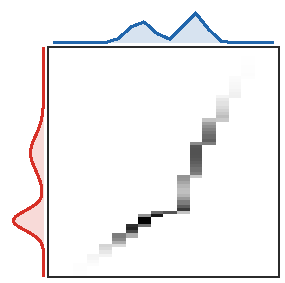
\includegraphics[width=.22\linewidth]{figures/kantorovich-discrete-gluing-lemma/ab-plan.pdf} &
\index{gluing lemma}% strictindex
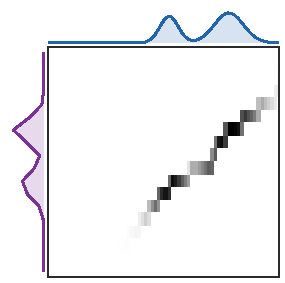
\includegraphics[width=.22\linewidth]{figures/kantorovich-discrete-gluing-lemma/bc-plan.pdf} &
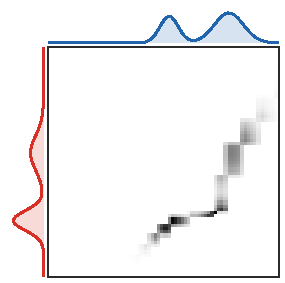
\includegraphics[width=.22\linewidth]{figures/kantorovich-discrete-gluing-lemma/glued-ac-plan.pdf} &
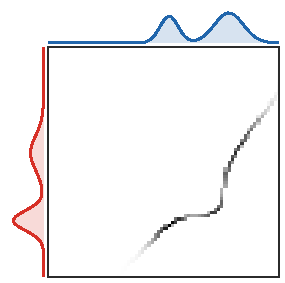
\includegraphics[width=.22\linewidth]{figures/kantorovich-discrete-gluing-lemma/direct-ac-plan.pdf}
\end{tabular}
\caption{\emph{Discrete gluing lemma in matrix form.} The first two panels are optimal one-dimensional couplings through an intermediate marginal $\b$. The third panel shows the induced marginal $\R=\P\diag(1/\b)\Q$ between $\a$ and $\VectMode{c}$; it is feasible and is the coupling used in the triangle-inequality proof. Because the intermediate marginal is represented on a coarser grid, the glued coupling is more mediated than the direct optimal coupling shown on the right. The thin box frames only the coupling matrix in each panel, while the attached marginal strips remain outside it.}
\label{fig:kantorovich-discrete-gluing-lemma}
\end{figure}

% We first consider the case where, using a term first introduce by~\cite{RubTomGui00}, the ``ground metric'' matrix $\C$ is fixed, representing substitution costs between bins, and shared across several histograms we would like to compare. The following proposition states that OT provides a meaningful distance between histograms supported on these bins.

When the cost matrix is the $p$th power of a distance matrix, the discrete Kantorovich value becomes a metric on histograms.

\begin{defn}[Discrete Wasserstein distance]\label{def-discrete-wasserstein-distance}
\index{Wasserstein!distance}% strictindex
	Let $\distD\in\RR_+^{n\times n}$ be a distance matrix on $\range{n}$ and let $p\geq1$. The discrete $p$-Wasserstein distance between histograms $\a,\b\in\simplex_n$ is
	\eql{\label{eq-wass-p-disc}
		\WassD_p(\a,\b) \eqdef \MKD_{\distD^p}(\a,\b)^{1/p}.
	}
	It depends on the chosen ground distance $\distD$.
\end{defn}

\begin{prop}[Metric property of discrete Wasserstein distance]\label{prop-metric-histo}
\index{Wasserstein!distance}% strictindex
	For every distance matrix $\distD$ on $\range{n}$, Definition~\ref{def-discrete-wasserstein-distance} defines a distance on $\simplex_n$: $\WassD_p$ is symmetric, positive, $\WassD_p(\a,\b)=0$ if and only if $\a = \b$, and it satisfies the triangle inequality
\index{triangle inequality}% strictindex
\eq{
	\foralls \a,\b,\VectMode{c} \in \simplex_n, \quad \WassD_p(\a,\VectMode{c}) \leq \WassD_p(\a,\b) + \WassD_p(\b,\VectMode{c}).
}
\end{prop}

\begin{proof}
	Transposition maps $\CouplingsD(\a,\b)$ bijectively onto $\CouplingsD(\b,\a)$ and preserves the cost because $\distD$ is symmetric. This proves symmetry. If $\a=\b$, the diagonal coupling $\diag(\a)$ has zero cost. Conversely, if an admissible coupling has zero cost, every off-diagonal entry must vanish because $\distD_{ij}>0$ for $i\neq j$. The coupling is therefore diagonal, and its two marginals coincide. This proves definiteness.

	For the triangle inequality, let $\P\in\CouplingsD(\a,\b)$ and $\Q\in\CouplingsD(\b,\VectMode{c})$ be optimal. Lemma~\ref{lem-gluing-discr} provides $\S\in\RR_+^{n\times n\times n}$ with these two marginals. Its first-third marginal
	\(\R_{ik}=\sum_j\S_{ijk}\)
	belongs to $\CouplingsD(\a,\VectMode{c})$. The ground-metric triangle inequality and Minkowski's inequality give
	\index{triangle inequality}% strictindex
	\index{gluing lemma}% strictindex
	\[
	\begin{aligned}
	\WassD_p(\a,\VectMode{c})
	&\leq \left(\sum_{i,j,k}\distD_{ik}^p\S_{ijk}\right)^{1/p}\\
	&\leq \left(\sum_{i,j,k}(\distD_{ij}+\distD_{jk})^p\S_{ijk}\right)^{1/p}\\
	&\leq \left(\sum_{i,j,k}\distD_{ij}^p\S_{ijk}\right)^{1/p}
	+\left(\sum_{i,j,k}\distD_{jk}^p\S_{ijk}\right)^{1/p}\\
	&=\WassD_p(\a,\b)+\WassD_p(\b,\VectMode{c}).
	\end{aligned}
	\]
	\index{Minkowski inequality}% strictindex
\end{proof}

\paragraph{Continuous gluing.}
\index{gluing lemma}% strictindex

Proposition~\ref{prop-metric-histo} generalizes from histogram to arbitrary measures that need not be discrete. For this, one needs the following general gluing lemma.
\index{histogram}% strictindex

\begin{lem}[Gluing lemma]\label{lem-gluing-general}
		Let $(\al,\be,\ga) \in \Mm_+^1(\Xx) \times \Mm_+^1(\Yy) \times \Mm_+^1(\Zz)$, where $\Xx$, $\Yy$ and $\Zz$ are Polish spaces in the sense of Definition~\ref{def-polish-metric-space}.
\index{Polish space}% strictindex
	%
		Given $\pi \in \Couplings(\al,\be)$ and $\xi \in \Couplings(\be,\ga)$, there exists a probability measure
\index{coupling measure}% strictindex
		$\sigma \in \Mm_+^1(\Xx \times \Yy \times \Zz)$ such that
	\eq{
		(P_{\Xx,\Yy})_\sharp \sigma = \pi
		\qandq
		(P_{\Yy,\Zz})_\sharp \sigma = \xi
	}
		where $P_{\Xx,\Yy}(x,y,z)=(x,y)$ and $P_{\Yy,\Zz}(x,y,z)=(y,z)$ are the coordinate projections.
\end{lem}
\begin{proof}
		Disintegrate the two couplings with respect to their common marginal $\be$:
\index{conditional!probability}% strictindex
\index{disintegration}% strictindex
		\[
			\pi(\d x,\d y)=\pi_y(\d x)\be(\d y),
			\qquad
			\xi(\d y,\d z)=\be(\d y)\xi_y(\d z).
		\]
		The Polish hypotheses guarantee the existence of the probability kernels $y\mapsto\pi_y$ and $y\mapsto\xi_y$. Define their conditional product by
		\[
			\int g\,\d\sigma
			\eqdef
			\int_\Yy\int_\Xx\int_\Zz
			g(x,y,z)\,\xi_y(\d z)\pi_y(\d x)\be(\d y)
		\]
		for every bounded Borel function $g$. Taking $g(x,y,z)=h(x,y)$ recovers $\pi$, while taking $g(x,y,z)=h(y,z)$ recovers $\xi$, proving the two marginal identities.

		In the discrete setting, $\pi_{y_j}=\sum_i(\P_{ij}/\b_j)\de_{x_i}$ and $\xi_{y_j}=\sum_k(\Q_{jk}/\b_j)\de_{z_k}$ whenever $\b_j>0$. Hence
		\[
			\sigma
			=
			\sum_{i,j,k}\S_{ijk}\de_{(x_i,y_j,z_k)},
			\qquad
			\S_{ijk}=\frac{\P_{ij}\Q_{jk}}{\b_j},
		\]
		with the value zero when $\b_j=0$, exactly as in~\eqref{eq-glued-discr}.
\end{proof}

Finite moments provide the natural domain for metric transport costs.
\begin{defn}[$p$-Wasserstein space]\label{def-p-wasserstein-space}
Let $(\Xx,d)$ be Polish, let $p\geq1$, and fix $x_0\in\Xx$. The $p$-Wasserstein space is
\[
	\Pp_p(\Xx)
	\eqdef
	\enscond{\al\in\Mm_+^1(\Xx)}{\int d(x,x_0)^p\d\al(x)<+\infty},
\]
which is independent of the choice of $x_0$.
\end{defn}
If $\al,\be\in\Pp_p(\Xx)$, then the product coupling has finite $p$-cost by the triangle inequality, so the Kantorovich value is finite. Proposition~\ref{prop-kantorovich-existence-compact} supplies an optimal coupling because $d^p$ is continuous and nonnegative~\cite{Villani09,SantambrogioBook}.
\index{triangle inequality}% strictindex
\index{tightness}% strictindex
\index{product!coupling}% strictindex

Using this gluing lemma, we can now construct the Wasserstein distance in the general setting of arbitrary distributions on a Polish space.
\index{Wasserstein!distance}% strictindex
\index{gluing lemma}% strictindex
\index{Polish space}% strictindex

\begin{defn}[Wasserstein distance]\label{def-wasserstein-distance}
Let $(\X,\dist)$ be a Polish metric space and $p\geq1$. On the space $\Pp_p(\X)$ of Definition~\ref{def-p-wasserstein-space}, the $p$-Wasserstein distance is
	\eql{\label{eq-defn-wass-dist}
		\Wass_p(\al,\be) \eqdef \MK_{\dist^p}(\al,\be)^{1/p}
		=
		\left(\inf_{\pi\in\Couplings(\al,\be)}
		\int_{\X\times\X}\dist(x,y)^p\d\pi(x,y)\right)^{1/p}.
	}
	It depends on the ground distance $\dist$.
\end{defn}

The Euclidean quadratic case separates the displacement of the means from the transport of the centered shapes. For general $p$, the same argument still gives a lower bound by the mean displacement.

\begin{prop}[Euclidean mean bound and quadratic decomposition]\label{prop-wasserstein-mean-decomposition}
\index{Wasserstein!distance}% strictindex
\index{mean!Wasserstein decomposition}% strictindex
\index{centered measure}% strictindex
	Let $p\geq1$ and $\al,\be\in\Pp_p(\RR^d)$, and denote their means by
	\[
		m_\al\eqdef\int_{\RR^d}x\,\d\al(x),
		\qquad
		m_\be\eqdef\int_{\RR^d}x\,\d\be(x).
	\]
	Then
	\[
		\norm{m_\al-m_\be}\leq\Wass_p(\al,\be).
	\]
	For $p=2$, define the centered translates
	\[
		\al^0\eqdef(x\mapsto x-m_\al)_\sharp\al,
		\qquad
		\be^0\eqdef(y\mapsto y-m_\be)_\sharp\be.
	\]
	Then the following exact decomposition holds:
	\[
		\Wass_2^2(\al,\be)
		=
		\norm{m_\al-m_\be}^2+\Wass_2^2(\al^0,\be^0).
	\]
\end{prop}
\begin{proof}
	For every $\pi\in\Couplings(\al,\be)$,
	\[
		m_\al-m_\be=\int_{\RR^d\times\RR^d}(x-y)\,\d\pi(x,y).
	\]
	Jensen's inequality therefore gives
	\[
		\norm{m_\al-m_\be}
		\leq
		\left(\int\norm{x-y}^p\,\d\pi(x,y)\right)^{1/p}.
	\]
	Taking the infimum over $\pi$ proves the first claim.

	For $p=2$, set
	\[
		\pi^0
		\eqdef
		\bigl((x,y)\mapsto(x-m_\al,y-m_\be)\bigr)_\sharp\pi.
	\]
	This translation defines a bijection from
	$\Couplings(\al,\be)$ onto $\Couplings(\al^0,\be^0)$. Writing
	$u=x-m_\al$ and $v=y-m_\be$, one has
	\[
		\int\norm{x-y}^2\,\d\pi
		=
		\norm{m_\al-m_\be}^2+\int\norm{u-v}^2\,\d\pi^0(u,v),
	\]
	because $\int(u-v)\,\d\pi^0(u,v)=0$. Taking the infimum over the corresponding couplings proves the decomposition.
\end{proof}

\begin{example}[Application to gene-expression distances]\label{ex-gene-expression-distance}
\index{single-cell genomics}% strictindex
\index{ground metric learning}% strictindex
	A single cell can be encoded as a measure over genes,
	\[
		\al_{\mathrm{cell}}=\sum_g e_g\de_{\varphi(g)},
	\]
	where \(e_g\geq0\), \(\sum_g e_g=1\), and \(\varphi(g)\) is a gene embedding or annotation vector. Wasserstein distances then compare cells by moving expression mass between genes. The choice of \(\dist(\varphi(g),\varphi(g'))\) is biologically meaningful: it can come from annotations, pathways or a learned ground metric. This is the idea behind the Gene Mover's Distance and related metric-learning approaches for single-cell data~\cite{BellazziCodegoniGualandiNicoraVercesi2021GeneMover,HuizingCantiniPeyre2021WassersteinSingularVectors}; it is the single-cell analogue of the cost-learning question revisited in Section~\ref{sec-metric-learning-inverse-ot}.
\end{example}

Single-cell OT also has a complementary population-level interpretation: instead of representing one cell as a measure over genes, one treats every cell as one atom of a time-indexed population law. Figure~\ref{fig:kantorovich-waddington-ot} follows the visualization introduced for Waddington-OT by Schiebinger et al.~\cite{schiebinger2017reconstruction}. Because single-cell sequencing is destructive, the coupling encodes inferred ancestor--descendant relations between consecutive populations rather than tracks of individually observed cells.

To make this construction precise, let \(\a_C\) be uniform on the labeled source set \(C\), and let \(\b_A,\b_B\) be uniform on the labeled target regions. For the released transport matrix \(\P\), the displayed descendant and ancestor laws are
\[
	\b_C^{\mathrm{desc}}
	=
	\frac{\P^\top\a_C}{\langle\P^\top\a_C,\ones\rangle},
	\qquad
	\a_R^{\mathrm{anc}}
	=
	\frac{\P\b_R}{\langle\P\b_R,\ones\rangle},
	\quad R\in\{A,B\}.
\]
Thus the plan, not the two-dimensional embedding, propagates probabilities. For this compact illustration, \(A\) and \(B\) are separated target regions whose pulled-back laws retain nontrivial overlap, and \(C\) is selected inside their common-ancestor region. Their common part is the componentwise minimum \(\a_{\cap}^{\mathrm{anc}}=\min\{\a_A^{\mathrm{anc}},\a_B^{\mathrm{anc}}\}\).
\index{Waddington-OT}% strictindex

\begin{figure}[htbp]
\centering
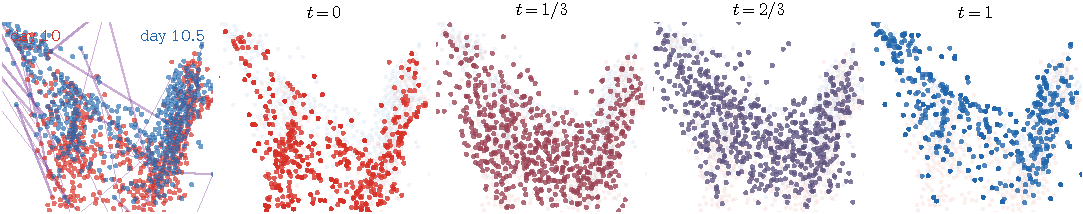
\includegraphics[width=.98\linewidth]{figures/kantorovich-waddington-ot/waddington-ot.pdf}
\caption{\emph{Waddington-OT between consecutive single-cell snapshots.} Every panel uses the official force-layout embedding, with the complete reprogramming landscape sampled in gray. The first overlays day-10 cells in red and day-10.5 cells in blue. Black rims and labels identify the conditioning sets: the second panel pushes \(C\) forward to its descendants, while the third pulls \(A\) backward to its ancestors. The last compares the ancestors of \(A\) and \(B\): red and blue encode the two exclusive parts, and violet their pointwise common part. Marker intensity and size encode normalized transported mass. The embedding is only a display plane; the released plan uses local 30-dimensional PCA costs.}
\index{single-cell genomics}% strictindex
\index{trajectory inference}% strictindex
\label{fig:kantorovich-waddington-ot}
\end{figure}

\begin{example}[Application to word embeddings and documents]\label{ex-word-mover-distance}
\index{word mover's distance}% strictindex
\index{natural language processing}% strictindex
	A document can similarly be viewed as a probability measure on a word-embedding space,
	\[
		\al_{\mathrm{doc}}=\sum_{w\in\mathrm{doc}} a_w\de_{e_w}.
	\]
	Here \(a_w\) are normalized word frequencies and \(e_w\) are word embeddings. The Word Mover's Distance is the Wasserstein distance between such document measures~\cite{kusner2015word}. It compares bags of words through the geometry learned by the embedding, so that replacing a word by a nearby synonym is less costly than replacing it by an unrelated word. When two embedding spaces are not already aligned, Gromov--Wasserstein variants compare their intrinsic neighborhood geometry instead of relying on a common coordinate system~\cite{alvarez2018towards}; this is the intrinsic-space viewpoint developed in Section~\ref{sec-gromov-wasserstein}.
\end{example}

\begin{prop}[Metric property of the Wasserstein distance]\label{prop-metric-measure}
\index{Wasserstein!distance}% strictindex
	Definition~\ref{def-wasserstein-distance} defines a distance on $\Pp_p(\X)$: $\Wass_p$ is symmetric and nonnegative, $\Wass_p(\al,\be)=0$ if and only if $\al=\be$, and
\index{triangle inequality}% strictindex
\eq{
	\foralls (\al,\be,\ga)\in\Pp_p(\X)^3, \qquad
	\Wass_p(\al,\ga)\leq\Wass_p(\al,\be)+\Wass_p(\be,\ga).
}
\end{prop}

\begin{proof}
	The value is finite on $\Pp_p(\X)$ because the product coupling has finite $p$-cost. If $\tau(x,y)=(y,x)$ is the flip map, then $\tau_\sharp\pi\in\Couplings(\be,\al)$ whenever $\pi\in\Couplings(\al,\be)$, and the transport cost is unchanged. This proves symmetry. The diagonal coupling $(\Id,\Id)_\sharp\al$ proves $\Wass_p(\al,\al)=0$.

	Conversely, Proposition~\ref{prop-kantorovich-existence-compact} supplies an optimal coupling $\pi$. If $\Wass_p(\al,\be)=0$, then $\dist(x,y)=0$ for $\pi$-almost every $(x,y)$, so $x=y$ almost surely under $\pi$. For every bounded Borel function $f$,
\index{optimal coupling}% strictindex
	\[
		\int f\,\d\al
		=
		\int f(x)\,\d\pi(x,y)
		=
		\int f(y)\,\d\pi(x,y)
		=
		\int f\,\d\be,
	\]
	and therefore $\al=\be$.

	For the triangle inequality, consider optimal couplings $\pi\in\Couplings(\al,\be)$ and $\xi\in\Couplings(\be,\ga)$,
\index{triangle inequality}% strictindex
	and glue them into $\sigma$ by Lemma~\ref{lem-gluing-general}. Let $P_{1,3}(x,y,z)=(x,z)$ and define $\eta\eqdef(P_{1,3})_\sharp\sigma$. Then $\eta\in\Couplings(\al,\ga)$. If the two original couplings are induced by maps $T_1$ and $T_2$, this construction is induced by $T_2\circ T_1$; gluing therefore extends composition of deterministic maps.
\index{Monge!problem}% strictindex
	The triangle inequality and Minkowski's inequality give
\index{Minkowski inequality}% strictindex
	\[
	\begin{aligned}
		\Wass_p(\al,\ga)
		&\leq\left(\int\dist(x,z)^p\d\sigma(x,y,z)\right)^{1/p}\\
		&\leq\left(\int(\dist(x,y)+\dist(y,z))^p\d\sigma(x,y,z)\right)^{1/p}\\
		&\leq\left(\int\dist(x,y)^p\d\sigma(x,y,z)\right)^{1/p}
		+\left(\int\dist(y,z)^p\d\sigma(x,y,z)\right)^{1/p}\\
		&=\left(\int_{\X\times\X}\dist(x,y)^p\d\pi(x,y)\right)^{1/p}
		+\left(\int_{\X\times\X}\dist(y,z)^p\d\xi(y,z)\right)^{1/p}\\
		&=\Wass_p(\al,\be)+\Wass_p(\be,\ga).
	\end{aligned}
	\]
\end{proof}

\begin{rem}[Gluing is the metric engine]\label{rem-gluing-metric-engine}
\index{gluing lemma}% strictindex
\index{metric!triangle inequality}% strictindex
	The proof above is the prototype for many metric constructions in the book. The only genuinely transport-specific step is the gluing lemma, Lemma~\ref{lem-gluing-general}: two couplings sharing a marginal can be lifted to a joint law, and the ordinary triangle inequality is then applied pointwise before integrating. The same pattern already appeared in the discrete proof of Proposition~\ref{prop-metric-histo}, where the glued tensor is written explicitly in \eqref{eq-glued-discr}. It reappears whenever a new distance is built from transport: quotient Wasserstein uses the same metric inheritance after optimizing over a group action in Proposition~\ref{prop-quotient-wasserstein-metric}; conditional Wasserstein glues fiberwise couplings in Proposition~\ref{prop-conditional-wasserstein-distance} and along geodesics in Proposition~\ref{prop-conditional-wasserstein-geodesics}; the conic construction of unbalanced OT uses gluing on cone couplings in Proposition~\ref{prop-homogeneous-unbalanced}; and the Gromov--Wasserstein metric theorem, Theorem~\ref{thm-gw-metric}, is the intrinsic-space analogue where couplings are glued while controlling pairwise distortions. In this sense, gluing is the metric engine behind most extensions of \(\Wass_p\), not merely a technical lemma for \eqref{eq-defn-wass-dist}.
\end{rem}

\paragraph{Interpolation induced by an optimal plan.}
\index{plan!interpolation}% strictindex
\label{sec-kantorovich-plan-interpolation}

The quadratic Wasserstein distance does not only compare two endpoint measures. An optimal plan also says how to move mass between them: each active pair $(x,y)$ travels along the segment joining $x$ to $y$. This turns an optimal coupling into a curve of measures.
\index{optimal coupling}% strictindex
\index{Wasserstein!distance}% strictindex

\begin{defn}[$\Wass_2$ geodesic induced by an optimal plan]\label{def-w2-geodesic-induced-by-plan}
\index{Wasserstein!geodesic}% strictindex
\index{plan!optimal}% strictindex
\index{McCann!interpolation}% strictindex
	Let $\al_0,\al_1\in\Pp_2(\RR^d)$, and let $\pi^\star\in\Couplings(\al_0,\al_1)$ be optimal for $\Wass_2^2(\al_0,\al_1)$. For $t\in[0,1]$, define
	\[
		e_t(x,y)\eqdef(1-t)x+t y,
		\qquad
		\al_t\eqdef(e_t)_\sharp\pi^\star .
	\]
	The curve $(\al_t)_{t\in[0,1]}$ is the displacement, or McCann, $\Wass_2$ geodesic induced by $\pi^\star$.
\end{defn}
In the discrete case, each mass $\P_{ij}$ moves from $x_i$ to $y_j$ along its own segment. When the optimal plan is not induced by a map, one source atom can split into several moving atoms. If the optimal plan is not unique, different optimal plans may also induce different $\Wass_2$ geodesics.
\index{discrete!measure}% strictindex
\index{plan!transport}% strictindex

\begin{prop}[Optimal-plan interpolation is a $\Wass_2$ geodesic]\label{prop-plan-interpolation-w2-geodesic}
\index{Wasserstein!geodesic}% strictindex
\index{constant-speed geodesic}% strictindex
	Let $(\al_t)_{t\in[0,1]}$ be defined by Definition~\ref{def-w2-geodesic-induced-by-plan}. Then, for every $0\leq s\leq t\leq1$,
	\[
		\Wass_2(\al_s,\al_t)
		=
		(t-s)\Wass_2(\al_0,\al_1).
	\]
	Thus $t\mapsto\al_t$ is a constant-speed geodesic for the metric $\Wass_2$.
\end{prop}
\begin{proof}
	Push the optimal plan $\pi^\star$ forward by $(e_s,e_t)$. This gives a coupling $\gamma_{s,t}\in\Couplings(\al_s,\al_t)$, and
	\[
		\int \norm{z-z'}^2\d\gamma_{s,t}(z,z')
		=
		\int \norm{e_t(x,y)-e_s(x,y)}^2\d\pi^\star(x,y)
		=
		(t-s)^2\Wass_2^2(\al_0,\al_1).
	\]
	Hence $\Wass_2(\al_s,\al_t)\leq(t-s)\Wass_2(\al_0,\al_1)$. Applying this upper bound to the three pairs $(0,s)$, $(s,t)$ and $(t,1)$, and using the triangle inequality of Proposition~\ref{prop-metric-measure}, gives
	\[
		\Wass_2(\al_0,\al_1)
		\leq
		\Wass_2(\al_0,\al_s)+\Wass_2(\al_s,\al_t)+\Wass_2(\al_t,\al_1)
		\leq
		\Wass_2(\al_0,\al_1).
	\]
	All inequalities are therefore equalities, in particular the middle segment has the claimed length.
\end{proof}

Figure~\ref{fig:kantorovich-plan-interpolation} visualizes the construction when the optimal plan splits mass, so that the intermediate measure is obtained by moving every coupled pair along its Euclidean segment.

\begin{figure}[H]
\centering
\begin{tabular}{@{}ccccc@{}}
\small $t=0$ & \small $t=1/4$ & \small $t=1/2$ & \small $t=3/4$ & \small $t=1$ \\[-.15em]
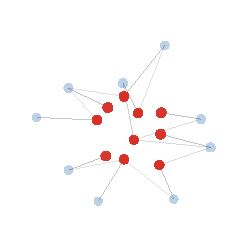
\includegraphics[width=.17\linewidth]{figures/kantorovich-plan-interpolation/time-000.pdf} &
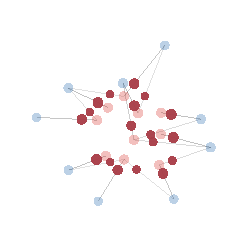
\includegraphics[width=.17\linewidth]{figures/kantorovich-plan-interpolation/time-025.pdf} &
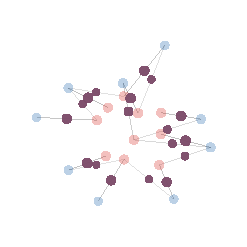
\includegraphics[width=.17\linewidth]{figures/kantorovich-plan-interpolation/time-050.pdf} &
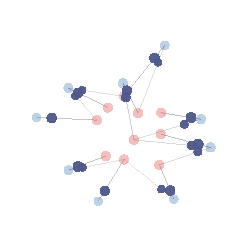
\includegraphics[width=.17\linewidth]{figures/kantorovich-plan-interpolation/time-075.pdf} &
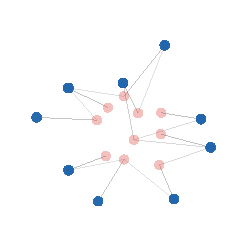
\includegraphics[width=.17\linewidth]{figures/kantorovich-plan-interpolation/time-100.pdf}
\end{tabular}
\caption{\emph{McCann interpolation induced by a non-deterministic optimal transport plan.} In every panel, the red and blue endpoint measures are shown with low opacity, thin gray segments display the support $\P_{ij}>\mathrm{tol}$ of the coupling, and the moving atoms are colored from red to blue along the interpolation.}
\index{McCann!interpolation}% strictindex
\index{plan!transport}% strictindex
\label{fig:kantorovich-plan-interpolation}
\end{figure}

\paragraph{General geodesic spaces.}
\index{geodesic!space}% strictindex
For Dirac masses in Euclidean space, the $\Wass_2$ geodesic from $\de_x$ to $\de_y$ is $t\mapsto\de_{(1-t)x+t y}$. The same idea extends to any geodesic metric space $(\X,\dist)$, meaning that each pair of points can be joined by a constant-speed metric geodesic. For each pair $(x,y)$, one replaces the Euclidean segment by a curve $\gamma^{x,y}:[0,1]\to\X$ such that $\gamma^{x,y}_0=x$, $\gamma^{x,y}_1=y$, and
\[
	\dist(\gamma^{x,y}_s,\gamma^{x,y}_t)=|t-s|\dist(x,y).
\]
If this geodesic is unique and depends measurably on $(x,y)$, one defines $e_t(x,y)=\gamma^{x,y}_t$ and sets $\al_t=(e_t)_\sharp\pi^\star$ for an optimal coupling $\pi^\star$. When geodesics are not unique, there is no canonical interpolation of a pair of Diracs unless a choice is made: one may select a particular geodesic between $x$ and $y$, or randomize among several such geodesics. The intrinsic formulation is to choose a probability measure $\eta$ on the path space of constant-speed geodesics, called a dynamical optimal plan, such that $(e_0,e_1)_\sharp\eta$ is an optimal coupling, and to set $\al_t=(e_t)_\sharp\eta$. Different measurable choices, or different conditional distributions over geodesics with the same endpoints, can give different $\Wass_2$ geodesics; the constant-speed identity remains the same. This path-space viewpoint is standard in the general theory of Wasserstein spaces~\cite{ambrosio2006gradient,Villani09,SantambrogioBook}.
\index{Dirac mass}% strictindex
\index{path space}% strictindex
\index{dynamical optimal plan}% strictindex


\paragraph{Comparison with Monge.}
\index{Monge!problem}% strictindex

	This distance $\Wass_p$ defined through the Kantorovich problem~\eqref{eq-defn-wass-dist} should be contrasted with the directed distance $\tilde\Wass_p$ obtained using Monge's problem~\eqref{eq-monge-distance}. The Kantorovich feasible set is never empty, since it contains the product coupling, although the $p$-cost may still be infinite without moment assumptions on non-compact spaces. By contrast, Monge's constraint set $\enscond{T}{T_\sharp \al=\be}$ can be empty. When an optimal Monge map exists, Kantorovich gives the same value by choosing the graph coupling $(\Id,T)_\sharp\al$.
\index{Kantorovich!problem}% strictindex
\index{product!coupling}% strictindex
\index{Monge!distance}% strictindex

The next proposition makes precise one important sense in which Kantorovich is the relaxation of Monge: when the source is atomless, allowing arbitrary couplings does not change the infimum value, although it may create an optimizer when no optimal map exists.
\index{graph!coupling}% strictindex
\index{lower semicontinuous envelope}% strictindex

\begin{prop}[Kantorovich as the plan-space relaxation of Monge]\label{prop-kantorovich-relaxation-monge}
\index{Kantorovich!relaxation}% strictindex
\index{Monge!problem}% strictindex
\index{measure!atomless}% strictindex
	Let $(\Xx,\dist)$ be a compact metric space, let $p\geq1$, and let $\al,\be\in\Pp(\Xx)$ with $\al$ atomless. Then
	\[
		\Wass_p(\al,\be)^p
		=
		\inf_{T_\sharp\al=\be}\int_\Xx \dist(x,T(x))^p\d\al(x).
	\]
	The infimum on the Monge side need not be attained.
\end{prop}
\begin{proof}
	Let $\pi\in\Couplings(\al,\be)$. Choose finite Borel partitions $(A_i)_i$ and $(B_j)_j$ of $\Xx$ whose cells have diameter at most $\varepsilon$. Set $m_{ij}=\pi(A_i\times B_j)$. Since $\al$ is atomless and $\sum_j m_{ij}=\al(A_i)$, each $A_i$ can be partitioned into Borel sets $A_{ij}$ with $\al(A_{ij})=m_{ij}$. If $m_{ij}>0$, then $\be(B_j)>0$, and Proposition~\ref{prop-existence-transport-map-atomless} gives a measurable map
	\[
		T_{ij}:A_{ij}\to B_j,
		\qquad
		(T_{ij})_\sharp\frac{\al|_{A_{ij}}}{m_{ij}}
		=
		\frac{\be|_{B_j}}{\be(B_j)}.
	\]
	Define $T$ by $T=T_{ij}$ on $A_{ij}$, ignoring null cells. Then $T_\sharp\al=\be$, because the contributions landing in $B_j$ sum to $\be|_{B_j}$, and the graph coupling $(\Id,T)_\sharp\al$ has the same masses $m_{ij}$ as $\pi$ on all rectangles $A_i\times B_j$.

	Let $h\in\Cc(\Xx\times\Xx)$. By uniform continuity on the compact product, the oscillation of $h$ on every rectangle $A_i\times B_j$ goes to zero as $\varepsilon\to0$. Since $\pi$ and $(\Id,T)_\sharp\al$ have the same mass on each rectangle, their integrals against $h$ differ by at most this maximal oscillation. Taking partitions with mesh tending to zero therefore gives graph couplings $(\Id,T_k)_\sharp\al$ converging weakly to $\pi$. Applying this to the continuous function $(x,y)\mapsto\dist(x,y)^p$ gives the convergence of costs.

	It remains to identify the relaxed functional. Define
	\[
		\mathcal G(\al,\be)
		\eqdef
		\enscond{(\Id,T)_\sharp\al}{T_\sharp\al=\be}
		\subset\Couplings(\al,\be),
		\qquad
		F_p(\pi)\eqdef\int_{\Xx\times\Xx}\dist(x,y)^p\d\pi(x,y),
	\]
	and let $G$ be the Monge graph functional which equals $F_p$ on $\mathcal G(\al,\be)$ and $+\infty$ otherwise. The function $F_p$ is weakly continuous on $\Couplings(\al,\be)$ and satisfies $F_p\leq G$. If $H$ is any weakly lower-semicontinuous function with $H\leq G$, then for the graph approximation above,
	\[
		H(\pi)\leq\liminf_k H((\Id,T_k)_\sharp\al)
		\leq
		\lim_k F_p((\Id,T_k)_\sharp\al)=F_p(\pi).
	\]
	Thus $F_p$ is the largest weakly lower-semicontinuous minorant of $G$, that is, the lower-semicontinuous envelope. Minimizing this envelope over all couplings gives the Kantorovich value, and the density argument gives the same infimum when restricting to graph couplings.
\end{proof}

Since $F_p$ is affine in the plan variable and $\Couplings(\al,\be)$ is convex, this envelope is also the closed convex relaxation of the Monge graph problem in the space of transport plans.
\index{convex!relaxation}% strictindex

At the level of endpoint measures, this gives the following literal lower-semicontinuous-envelope interpretation for the Monge $p$-cost, whenever source measures can be regularized into atomless ones.

\begin{cor}[Lower-semicontinuous envelope of the Monge \(p\)-cost]\label{cor-wasserstein-lsc-envelope-monge-distance}
\index{Monge!distance}% strictindex
\index{lower semicontinuous envelope}% strictindex
		Let $(\Xx,\dist)$ be a compact metric space and assume that atomless probability measures are dense in $\Pp(\Xx)$ for the $\Wass_p$ topology. Then $(\al,\be)\mapsto\Wass_p(\al,\be)^p$ is the lower-semicontinuous envelope, on $\Pp(\Xx)\times\Pp(\Xx)$ for the product $\Wass_p$ topology, of the extended Monge cost
	\[
		\tilde\Wass_p(\al,\be)^p
		=
		\inf_{\substack{T:\Xx\to\Xx\\ T_\sharp\al=\be}}
		\int_\Xx \dist(x,T(x))^p\d\al(x),
	\]
	with the convention $\tilde\Wass_p(\al,\be)^p=+\infty$ if no admissible map exists.
\end{cor}
\begin{proof}
	For every admissible map $T$, the graph plan $(\Id,T)_\sharp\al$ is a coupling, hence $\Wass_p(\al,\be)^p\leq \tilde\Wass_p(\al,\be)^p$. Since $\Wass_p^p$ is continuous for the product $\Wass_p$ topology, it is a lower-semicontinuous minorant of the extended Monge cost.

	Conversely, let $H$ be any lower-semicontinuous minorant of the extended Monge cost. Fix $(\al,\be)$ and choose atomless $\al_k\to\al$ in $\Wass_p$. By Proposition~\ref{prop-kantorovich-relaxation-monge}, $\tilde\Wass_p(\al_k,\be)^p=\Wass_p(\al_k,\be)^p$. Therefore
	\[
		H(\al,\be)
		\leq
		\liminf_k H(\al_k,\be)
		\leq
		\lim_k \Wass_p(\al_k,\be)^p
		=
		\Wass_p(\al,\be)^p.
	\]
	Thus no larger lower-semicontinuous minorant exists.
\end{proof}

The extra density assumption in the corollary is essential. If $\al$ has atoms, the graph-density statement can fail dramatically: for instance a single source Dirac mass cannot be mapped to two target Dirac masses. On finite spaces, the topology is discrete and this obstruction cannot be removed by closure. In such cases the Kantorovich formulation is not merely a closure of existing maps with the same marginals; it genuinely adds the possibility of splitting atomic mass.
\index{mass!splitting}% strictindex


%%%%
\section{Topology and Applications}
\label{sec-wasserstein-topology-applications}
\index{Wasserstein!distance}% strictindex

This section shifts from metric axioms to topology and uses. Wasserstein distances metrize weak convergence under moment control, sit between weak and strong topologies, and provide quantitative estimates in probability and robust optimization.
\index{weak!convergence}% strictindex

\paragraph{Convergence in law topology.}
\index{convergence!law}% strictindex

On a bounded metric space, all $\Wass_p$ distances define the same topology, although they are not equivalent as distances.

\begin{prop}[Comparison of Wasserstein distances on bounded spaces]\label{prop-comp-wass-p}
\index{Wasserstein!distance}% strictindex
		Let $(\Xx,\dist)$ be a bounded Polish metric space, let $1\leq p\leq q<\infty$, and let $\al,\be\in\Pp_q(\Xx)$. Then
		\eq{
			\Wass_p(\al,\be) \leq \Wass_q(\al,\be) \leq \operatorname{diam}(\Xx)^{\frac{q-p}{q}} \Wass_p(\al,\be)^{\frac{p}{q}},
			\qquad
			\operatorname{diam}(\Xx)\eqdef\sup_{x,y\in\Xx}\dist(x,y).
		}
\end{prop}
\begin{proof}
			The left inequality follows from Jensen's inequality, applied to any coupling $\pi$ and to the convex function $r\mapsto r^{q/p}$:
	\index{Jensen inequality}% strictindex
	\index{convex!function}% strictindex
			\eq{
				\pa{\int \dist(x,y)^{p} \d\pi(x,y)}^{\frac{q}{p}} \leq \int \dist(x,y)^{q} \d\pi(x,y).
			}
			Taking the infimum gives $\Wass_p\leq\Wass_q$. The right inequality follows from
			\(\dist(x,y)^q \leq \operatorname{diam}(\Xx)^{q-p} \dist(x,y)^p\)
			and taking the infimum over couplings once more.
		\end{proof}

The Wasserstein distance $\Wass_p$ is a weak distance: it compares singular distributions, such as discrete measures, and quantifies spatial shifts between supports. Its topology is studied in detail in~\cite{Villani09,SantambrogioBook,gigli2011user}, while empirical rates are quantified in~\cite{dudley1969speed,fournier2015rate,weed2017sharp,boissard2015distribution,bolley2007quantitative}.
\index{Wasserstein!distance}% strictindex

\begin{defn}[Weak, or narrow, topology]\label{dfn-weak-conv}
\index{topology!weak}% strictindex
		A sequence $(\al_k)_k$ converges weakly, or narrowly, to $\al$ in $\Mm_+^1(\Xx)$, denoted $\al_k \rightharpoonup \al$, if and only if
		\[
			\int_\Xx f\d\al_k\longrightarrow\int_\Xx f\d\al
			\qquad\text{for every }f\in\Cc_b(\Xx).
		\]
		On a compact space, $\Cc_b(\Xx)=\Cc(\Xx)$ and this is precisely weak$^*$ convergence in the duality between measures and continuous functions. The term weak$^*$ is therefore also used informally in the book when no confusion can arise.
\index{continuous!bounded function}% strictindex
\end{defn}

\begin{rem}[A Riemann-sum weak limit]\label{rem-riemann-weak-limit}
\index{Riemann sum}% strictindex
\index{weak!limit}% strictindex
	On $\Xx=\RR$, the empirical measures on a regular grid satisfy
\index{empirical!measure}% strictindex
	\[
		\frac{1}{n} \sum_{k=1}^n \de_{k/n} \rightharpoonup \Uu_{[0,1]}.
	\]
	Indeed, for every continuous bounded function $f$,
	\[
		\frac{1}{n} \sum_{k=1}^n f(k/n) \longrightarrow \int_0^1 f(x) \d x,
	\]
	which is precisely the convergence of Riemann sums. This convergence is weak but not strong: for every $n$, the discrete measure and the uniform density are mutually singular, hence their total variation distance is equal to $2$.
\index{Riemann sum}% strictindex
\index{total variation}% strictindex
\end{rem}

\begin{rem}[Weak convergence for discrete measures]\label{rem-weak-conv-disc}
\index{weak!convergence}% strictindex
\index{discrete!measure}% strictindex
	In the special case of a single Dirac, $\de_{x^{(n)}} \rightharpoonup \de_x$ is equivalent to $\int f \d\de_{x^{(n)}} = f(x^{(n)}) \rightarrow \int f \d\de_{x} = f(x)$ for any continuous $f$. This in turn is equivalent to $x^{(n)} \rightarrow x$.
	For a fixed number of atoms, if $\al_n=\sum_{i=1}^N a_i^{(n)}\de_{x_i^{(n)}}$ and, after extracting a subsequence and relabeling, $a_i^{(n)}\to a_i$ and $x_i^{(n)}\to x_i$, then $\al_n$ converges weakly to $\sum_i a_i\de_{x_i}$, with atoms at identical limits merged. Without a uniform bound on the number of atoms, weak limits of discrete measures can be non-discrete; empirical measures are the standard example.
\index{weak!limit}% strictindex
\index{empirical!measure}% strictindex
\end{rem}

In terms of random vectors, if $X_n \sim \al_n$ and $X \sim \al$ (not necessarily defined on the same probability space), weak convergence corresponds to convergence in law of $X_n$ toward $X$.
\index{convergence!in law}% strictindex
\index{weak!convergence}% strictindex

\begin{rem}[Modes of convergence for random variables]\label{rem-random-variable-convergences}
\index{random variable}% strictindex
\index{convergence!mode}% strictindex
	Convergence of laws should be distinguished from stronger notions of convergence for random variables. If $X_n$ and $X$ are defined on a common probability space, then $X_n\to X$ almost surely means pointwise convergence outside a null set, while convergence in probability means
\index{convergence!in probability}% strictindex
	\[
		\foralls \epsilon>0,\qquad
		\PP(\norm{X_n-X}>\epsilon)\to0.
	\]
	Almost-sure convergence implies convergence in probability, and convergence in probability implies convergence in law. Convergence in law is exactly weak, or narrow, convergence of the probability measures $(X_n)_\sharp\PP\rightharpoonup X_\sharp\PP$, and does not require all variables to live on the same probability space. Strong convergence of measures, for instance convergence in total variation, is different and usually much stronger: it controls the mass assigned to all measurable sets, not only averages against continuous test functions. In particular, total variation convergence implies weak convergence, but the converse fails for empirical approximations of continuous laws.
\index{convergence!in law}% strictindex
\index{probability measure}% strictindex
\index{weak!convergence}% strictindex
\index{total variation}% strictindex
\end{rem}

Convolution describes sums of independent random variables.
\begin{defn}[Convolution of measures]\label{def-measure-convolution}
	For probability measures $\al,\be$ on $\RR^d$, their convolution is
	\[
		\al*\be\eqdef\operatorname{add}_\sharp(\al\otimes\be),
		\qquad \operatorname{add}(x,y)=x+y.
	\]
	Equivalently, for every bounded continuous $\varphi$,
	\[
		\int\varphi\,\d(\al*\be)
		=
		\iint\varphi(x+y)\,\d\al(x)\d\be(y).
	\]
\end{defn}
Thus $\al*\be$ is the law of $X+Y$ when $X$ and $Y$ are independent with laws $\al$ and $\be$. When $\al=\density{\al}\d x$ and $\be=\density{\be}\d x$, their convolution has density
\[
	\density{\al*\be}(z)
	=
	(\density{\al}*\density{\be})(z)
	=
	\int_{\RR^d}\density{\al}(x)\density{\be}(z-x)\d x.
\]

\begin{rem}[Central limit theorem]\label{rem-clt}
\index{central limit theorem}% strictindex
	The central limit theorem states that if $(X_i)_{i\geq1}$ are i.i.d. random vectors with finite second moments, $\EE(X_i)=0$, and $\EE(X_i X_i^\top)=\Id$, then the normalized sum
	\[
		Z_n \eqdef \frac{1}{\sqrt{n}} \sum_{i=1}^n X_i
	\]
	converges in law toward the standard Gaussian $\Gaussian(0,\Id)$. In the terminology recalled above, this means that the measure $\al_n$ representing the law of $Z_n$ converges weakly toward the centered Gaussian measure $\al=\Gaussian(0,\Id)$.

	Equivalently, this is a statement about the convolution of Definition~\ref{def-measure-convolution}.
\index{measure convolution}% strictindex
	If $\al$ is the common law of the variables $X_i$, writing $\al^{*n}$ for the $n$-fold convolution of $\al$ with itself, and denoting by $D_a(x)=a x$ the dilation map, the law of $Z_n$ is
	\[
		\al_n=(D_{1/\sqrt n})_\sharp\al^{*n}.
	\]
	The CLT therefore says that the normalized $n$-fold convolution $(D_{1/\sqrt n})_\sharp\al^{*n}$ converges weakly to the Gaussian $\Gaussian(0,\Id)$.
\index{measure convolution}% strictindex
\index{rescaled convolution}% strictindex
\end{rem}

Figure~\ref{fig:matching-quantitative-clt} makes this qualitative weak convergence visible in the elementary Bernoulli case: every finite-$n$ law is discrete, yet the normalized atom heights approach the Gaussian density.

\begin{figure}[H]
\centering
\begin{tabular}{@{}ccccc@{}}
\small $n=1$ & \small $n=2$ & \small $n=4$ & \small $n=16$ & \small $n=64$ \\[-.15em]
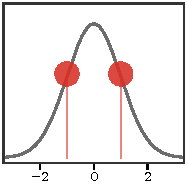
\includegraphics[width=.17\linewidth]{figures/matching-quantitative-clt/n-001.pdf} &
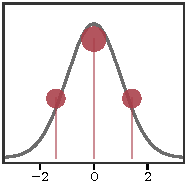
\includegraphics[width=.17\linewidth]{figures/matching-quantitative-clt/n-002.pdf} &
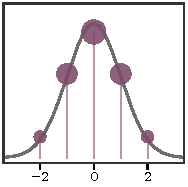
\includegraphics[width=.17\linewidth]{figures/matching-quantitative-clt/n-004.pdf} &
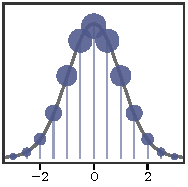
\includegraphics[width=.17\linewidth]{figures/matching-quantitative-clt/n-016.pdf} &
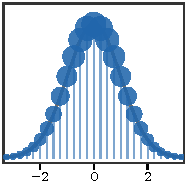
\includegraphics[width=.17\linewidth]{figures/matching-quantitative-clt/n-064.pdf}
\end{tabular}
\caption{\emph{Central-limit theorem for normalized Bernoulli sums.} Starting from $\al_0=\frac12(\delta_{-1}+\delta_1)$, the law of $Z_n=n^{-1/2}\sum_{i=1}^n X_i$ remains discrete, but its rescaled atom heights approach the standard Gaussian density shown in gray. Proposition~\ref{prop-berry-esseen-w1} later quantifies this weak convergence in $\Wass_1$.}
\index{central limit theorem}% strictindex
\index{weak!convergence}% strictindex
\label{fig:matching-quantitative-clt}
\end{figure}

\begin{rem}[A quantitative CLT in Wasserstein form]\label{rem-wasserstein-berry-esseen-pointer}
\index{Berry-Esseen!theorem}% strictindex
\index{central limit theorem!quantitative}% strictindex
\index{Wasserstein!distance}% strictindex
	The metric viewpoint on weak convergence is not only topological. It also turns some classical limit theorems into quantitative metric estimates. For instance, the Berry--Esseen theorem can be stated as a bound on the \(\Wass_1\) distance between the law of the normalized sum \(n^{-1/2}\sum_i X_i\) and the limiting Gaussian. By Kantorovich--Rubinstein duality, this is exactly a uniform control of the CLT error over all \(1\)-Lipschitz test functions. This application is developed later in Section~\ref{sec-law-large-numbers-clt}, see in particular Proposition~\ref{prop-berry-esseen-w1}.
\index{Kantorovich-Rubinstein@Kantorovich--Rubinstein!duality}% strictindex
\index{Lipschitz!test function}% strictindex
	\end{rem}

\paragraph{Strong versus weak topology.}
\index{topology!strong}% strictindex
\index{topology!weak}% strictindex
The total variation norm was introduced in Definition~\ref{defn-total-variation} and Proposition~\ref{prop-tv-dual-measure}. Its induced topology is often called the ``strong'' topology on measures. In the present section we only use the recall that, for a signed difference $\al-\be$,
\index{total variation}% strictindex
\[
	\norm{\al-\be}_{\TV}=|\al-\be|(\Xx),
\]
so densities give an $L^1$ norm and discrete signed measures give an $\ell^1$ norm of the signed weights.
\index{signed!measure}% strictindex

The following proposition shows that the TV norm can be seen as a Wasserstein distance, but for a ``degenerate'' 0/1 metric.
\index{Wasserstein!distance}% strictindex

\begin{prop}[Total variation as Wasserstein for the discrete metric]\label{prop-rel-wass-tv}
\index{total variation}% strictindex
		Let $\Xx$ be a standard Borel space, let $\al$ and $\be$ be probability measures on $\Xx$, and equip $\Xx$ with the $0/1$ cost $d_0(x,x)=0$ and $d_0(x,y)=1$ for $x\neq y$. Then, for every $p\geq1$,
		\eq{
			\inf_{\pi\in\Couplings(\al,\be)}\int d_0(x,y)^p\d\pi(x,y)
			=
			\frac{1}{2}\norm{\al-\be}_{\TV}.
		}
		Whenever the $0/1$ metric is used as the ground metric, the left-hand side is $\Wass_p(\al,\be)^p$.
\end{prop}
\begin{proof}
		Let $\lambda=\al+\be$, write $a=\d\al/\d\lambda$ and $b=\d\be/\d\lambda$, and define the common part $\eta$ by
		\(\frac{\d\eta}{\d\lambda}=\min(a,b)\).
		Its residuals $\al'=\al-\eta$ and $\be'=\be-\eta$ are mutually singular and have the same mass
		\[
			r
			=
			1-\eta(\Xx)
			=
			\frac12\int|a-b|\d\lambda
			=
			\frac12\norm{\al-\be}_{\TV}.
		\]
		For any $\pi\in\Couplings(\al,\be)$, define its diagonal submeasure by
		\(\zeta(A)=\pi\bigl(\{(x,x):x\in A\}\bigr)\).
		Then $\zeta\leq\al$ and $\zeta\leq\be$, so its density with respect to $\lambda$ is bounded by $\min(a,b)$. Consequently $\zeta\leq\eta$, hence $\pi(\{x=y\})\leq\eta(\Xx)$, and
		\[
			\int d_0(x,y)^p\d\pi(x,y)
			=
			1-\pi(\{x=y\})
			\geq r.
		\]
		If $r=0$, the diagonal coupling attains this bound. If $r>0$, let $\Delta(x)=(x,x)$ and set
		\[
			\pi^\star
			=
			\Delta_\sharp\eta+\frac{1}{r}\al^{\prime}\otimes\be^{\prime}.
		\]
		This is a coupling of $\al$ and $\be$. Since $\al'\perp\be'$, the product term is concentrated off the diagonal, so its $0/1$ cost is exactly its total mass $r$. Thus $\pi^\star$ attains the lower bound.
\end{proof}


As explained in Remark~\ref{rem-weak-conv-disc}, in the special case of Diracs, $\de_{x_n} \rightharpoonup \de_x$  is equivalent to $x_n \rightarrow x$. One can then contrast the strong topology with the Wasserstein distance if $x_n \neq x$,
\index{topology!strong}% strictindex
\index{Wasserstein!distance}% strictindex
\eq{
	\norm{\de_{x_n}-\de_x}_{\TV}=2
	\qandq
	\Wass_p(\de_{x_n},\de_x) = d(x_n,x).
}
Thus a moving Dirac sequence can converge in total variation only if it is eventually stationary, whereas it converges in Wasserstein distance whenever its locations converge. On an unbounded space, weak convergence alone does not prevent a vanishing amount of mass from escaping to infinity. Wasserstein convergence is exactly weak convergence supplemented by control of this moment tail.
\index{weak!convergence}% strictindex

\begin{prop}[Wasserstein convergence on Polish spaces]\label{prop-wass-topology-polish}
\index{Wasserstein!topology}% strictindex
	Let $(\Xx,d)$ be a Polish metric space, let $1\leq p<+\infty$, and let $\al_k,\al\in\Pp_p(\Xx)$. For any reference point $x_0\in\Xx$, the following are equivalent:
	\begin{enumerate}
		\item $\Wass_p(\al_k,\al)\to0$;
		\item $\al_k\rightharpoonup\al$ and the $p$th moments converge,
		\eq{
			\int d(x,x_0)^p\d\al_k(x)
			\longrightarrow
			\int d(x,x_0)^p\d\al(x);
		}
		\item $\al_k\rightharpoonup\al$ and the $p$th moments are uniformly integrable,
		\eq{
			\lim_{R\to+\infty}\sup_k
			\int_{\{d(x,x_0)>R\}}d(x,x_0)^p\d\al_k(x)=0.
		}
	\end{enumerate}
	These conditions do not depend on the choice of $x_0$.
\end{prop}
\begin{proof}
	Assume first that $\Wass_p(\al_k,\al)\to0$. Since $\Wass_1\leq\Wass_p$, integration against every bounded $1$-Lipschitz function converges; such functions determine weak convergence on Polish spaces. For any coupling $\pi\in\Couplings(\al_k,\al)$, the reverse triangle inequality in $L^p(\pi)$ gives
	\[
		\left|
		\left(\int d(x,x_0)^p\d\al_k(x)\right)^{1/p}
		-
		\left(\int d(y,x_0)^p\d\al(y)\right)^{1/p}
		\right|
		\leq
		\left(\int d(x,y)^p\d\pi(x,y)\right)^{1/p}.
	\]
	Taking the infimum over $\pi$ proves convergence of the $p$th moments, hence (ii).

	Conversely, assume (ii). By the Skorokhod representation theorem, there exist random variables $X_k\sim\al_k$ and $X\sim\al$ on a common probability space such that $X_k\to X$ almost surely. Consequently $d(X_k,x_0)^p\to d(X,x_0)^p$ almost surely, and the assumed convergence of their expectations implies, by Scheff\'e's lemma, convergence in $L^1$. In particular, the family $(d(X_k,x_0)^p)_k$ is uniformly integrable. Since
	\[
		d(X_k,X)^p
		\leq 2^{p-1}\bigl(d(X_k,x_0)^p+d(X,x_0)^p\bigr),
	\]
	the variables $d(X_k,X)^p$ are uniformly integrable and converge almost surely to zero. Vitali's theorem therefore gives $\EE[d(X_k,X)^p]\to0$. The law of $(X_k,X)$ is an admissible coupling, so
	\[
		\Wass_p(\al_k,\al)^p\leq\EE[d(X_k,X)^p]\longrightarrow0.
	\]

	It remains to compare (ii) and (iii). The preceding Skorokhod argument shows that (ii) makes $d(X_k,x_0)^p$ uniformly integrable, which is exactly the tail condition in (iii). Conversely, assume (iii) and define the bounded continuous truncation $h_R(x)=\min\{d(x,x_0)^p,R^p\}$. Weak convergence gives $\int h_R\d\al_k\to\int h_R\d\al$ for every $R$. The uniform tail bound in (iii), together with the integrability of $d(\cdot,x_0)^p$ under $\al$, then lets $R\to+\infty$ and proves convergence of the untruncated moments. This establishes all three equivalences. Since (i) is independent of the reference point, so are (ii) and (iii)~\cite{Villani09,SantambrogioBook,ambrosio2006gradient}.
\index{Wasserstein!distance}% strictindex
\index{weak!convergence}% strictindex
\index{uniform integrability}% strictindex
\index{moment!convergence}% strictindex
\end{proof}

On a compact metric space, the moment function $d(\cdot,x_0)^p$ is bounded and continuous, so weak convergence automatically implies moment convergence. Proposition~\ref{prop-wass-topology-polish} therefore recovers the familiar fact that $\Wass_p$ metrizes weak convergence on $\Pp(\Xx)$.

On a finite metric space, the strong and weak topologies coincide. The following quantitative comparison explains this equivalence.
\index{Wasserstein!distance}% strictindex
\index{topology!weak}% strictindex

\begin{prop}[Comparison with total variation on finite spaces]
\index{total variation}% strictindex
\index{discrete!space}% strictindex
		Let $(\Xx,d)$ be a finite metric space and define
		\eq{
			d_{\min} \eqdef \min_{x\neq y}d(x,y)>0,
			\qquad
			d_{\max} \eqdef \max_{x,y}d(x,y)<+\infty.
		}
		Then, for every $\al,\be\in\Pp(\Xx)$,
		\eq{
			\frac{d_{\min}}{2}\norm{\al-\be}_{\TV}
			\leq \Wass_1(\al,\be)
			\leq \frac{d_{\max}}{2}\norm{\al-\be}_{\TV}.
		}
\end{prop}

\begin{proof}
	We denote $d_0(x,y)$ the distance such that $d_0(x,x)=0$ and $d_0(x,y)=1$ for $x \neq y$. One has
	\(d_{\min} d_0(x,y) \leq d(x,y) \leq d_{\max} d_0(x,y)\),
	so that integrating this against any $\pi \in \Couplings(\al,\be)$ and taking the minimum among those $\pi$ gives the result using Proposition~\ref{prop-rel-wass-tv}.
\end{proof}

The constants are optimal: for $\al=\de_x$ and $\be=\de_y$ with $x\neq y$, the comparison reduces to
\eq{
	d_{\min} \leq d(x,y) \leq d_{\max}.
}
%
Choosing pairs that attain $d_{\min}$ or $d_{\max}$ gives equality in the corresponding bound. The comparison deteriorates as $d_{\max}/d_{\min}$ grows. On spaces with arbitrarily close distinct points, $d_{\min}=0$ and no such two-sided equivalence is possible, consistently with the difference between strong and weak convergence.
\index{topology!weak}% strictindex

\begin{example}[Application to single-cell trajectory inference]\label{ex-single-cell-trajectory-inference}
\index{single-cell genomics}% strictindex
\index{trajectory inference}% strictindex
	A single-cell time course gives empirical laws
	\[
		\al_{t_k}=\frac1{n_k}\sum_{i=1}^{n_k}\de_{x_i^{[k]}}
	\]
	on a gene-expression or latent cell-state space. Since sequencing is destructive, one observes populations at successive times, not trajectories of identical cells. Couplings \(\pi_k\in\Couplings(\al_{t_k},\al_{t_{k+1}})\) provide soft ancestor--descendant relations; Figure~\ref{fig:kantorovich-waddington-ot} visualizes one such consecutive coupling. After disintegration into Markov kernels, they can be chained to define population-level trajectories. This static sequence of couplings is the discrete-time shadow of the dynamic formulations of Chapter~\ref{sec-dynamic-optimal-transport}; entropic and unbalanced variants account for branching, noise and growth in modern single-cell models~\cite{schiebinger2017reconstruction,TongHuangWolfVanDijkKrishnaswamy2020TrajectoryNet,LavenantZhangKimSchiebinger2021TrajectoryInference,KleinUsciddaTheisCuturi2023GENOT}.
\end{example}

\section{Measure-to-Vector Maps on Wasserstein Space}\label{sec-measure-to-vector-maps}
\index{measure-to-vector map}% strictindex
\index{functional!on Wasserstein space}% strictindex
\index{Wasserstein!space}% strictindex

Many losses, statistics and observables depend on a probability law rather than on a single point. This section formalizes such measure-to-vector maps, introduces their natural metric regularity and shows how finite particle samples generate constructive polynomial approximations. Chapter~\ref{sec-wasserstein-gradient-flows} returns to scalar functionals as energies to be minimized over Wasserstein space.

\paragraph{Functionals and Wasserstein--H\"older regularity.}
\index{Wasserstein!H\"older functional}% strictindex

A scalar functional is a map
\[
	f:\Pp_p(\Xx)\longrightarrow\RR.
\]
There is no loss of principle in starting with scalar values. If \(F=(f_1,\ldots,f_s):\Pp_p(\Xx)\to\RR^s\), the definitions and constructions below apply coordinatewise, and the resulting bounds combine in any norm on \(\RR^s\). For the quantitative approximation results, assume from now on that \(\Xx\subset\RR^d\) is compact; in particular, \(\Pp_p(\Xx)=\Pp(\Xx)\).

\begin{defn}[Wasserstein--H\"older functional]\label{def-wasserstein-holder-functional}
	Let \(p\geq1\) and \(0<\eta\leq1\). A functional \(f:\Pp(\Xx)\to\RR\) is \(\eta\)-H\"older for \(\Wass_p\), with constant \(L\), if
	\begin{equation}\label{eq-wasserstein-holder-functional}
		|f(\al)-f(\be)|
		\leq
		L\Wass_p(\al,\be)^\eta
		\qquad
		\text{for all }\al,\be\in\Pp(\Xx).
	\end{equation}
\end{defn}

The endpoint \(\eta=1\) is Wasserstein--Lipschitz regularity. It is the natural stability assumption for a functional: perturbing the input law by a small transport cost changes its output by at most a proportional amount. The restriction \(\eta\leq1\) is intrinsic on a geodesic space. Indeed, subdividing a constant-speed geodesic into \(N\) pieces shows that a globally H\"older functional with exponent \(\eta>1\) is constant along that geodesic, hence constant when every pair of points can be joined by one.

\begin{rem}[$\Wass_2$-Lipschitz functionals and bounded gradients]\label{rem-w2-lipschitz-bounded-gradient}
\index{Wasserstein!Lipschitz functional}% strictindex
\index{Wasserstein!gradient}% strictindex
	An \(L\)-Lipschitz functional has descending metric slope at most \(L\). Conversely, on a geodesic metric space, if the slope is a strong upper gradient uniformly bounded by \(L\), integrating it along geodesics shows that the functional is \(L\)-Lipschitz. In the smooth Otto calculus on \(\Pp_2(\RR^d)\), this slope is the \(L^2(\al)\)-norm of the Wasserstein gradient introduced in Proposition~\ref{prop-formal-wass-gradient}:
	\[
		|\partial f|_{\Wass_2}(\al)
		=
		\norm{\Wgrad f(\al)}_{L^2(\al)} .
	\]
	Thus, under the usual chain-rule assumptions, the bound
	\[
		\sup_{\al}\norm{\Wgrad f(\al)}_{L^2(\al)}\leq L
	\]
	is the differential counterpart of \(\Wass_2\)-Lipschitz regularity. This should not be confused with smoothness in optimization, which controls variation of the gradient itself.
\end{rem}

\paragraph{Examples and non-examples.}
\index{relative entropy!regularity}% strictindex

Basic OT quantities already provide useful examples. For a fixed \(\be\in\Pp(\Xx)\), the triangle inequality shows that \(\al\mapsto\Wass_p(\al,\be)\) is \(1\)-Lipschitz. More generally, \(\al\mapsto\Wass_p(\al,\be)^\eta\) is \(\eta\)-H\"older with constant one, since \(|r^\eta-s^\eta|\leq|r-s|^\eta\) for \(r,s\geq0\). If \(V:\Xx\to\RR\) is \(L\)-Lipschitz, then Kantorovich--Rubinstein duality and \(\Wass_1\leq\Wass_p\) give
\[
	f(\al)=\int_{\Xx} V\,\d\al,
	\qquad
	|f(\al)-f(\be)|\leq L\Wass_p(\al,\be).
\]
Pointwise mass is a simple non-example. If \(x_0\) is a non-isolated point of \(\Xx\), choose \(x_n\to x_0\) with \(x_n\neq x_0\). Although \(\de_{x_n}\to\de_{x_0}\) in every \(\Wass_p\), the functional \(\al\mapsto\al(\{x_0\})\) jumps from zero to one. Relative entropy fails even more sharply on the full Wasserstein space. If \(\be\) is nonatomic and \(\widehat\be_n\) is its empirical measure, then \(\widehat\be_n\to\be\) in \(\Wass_p\) almost surely, whereas \(\KL(\widehat\be_n|\be)=+\infty\). Density-based functionals therefore require additional regularity assumptions or smoothing before one can expect Wasserstein--H\"older control.

\paragraph{Interaction polynomials.}
\index{interaction polynomial}% strictindex
\index{Wasserstein!polynomial}% strictindex

Finite-body interactions provide the natural polynomial functions of a measure. For a bounded continuous symmetric kernel \(\varphi_m:\Xx^m\to\RR\), define the interaction polynomial of order at most \(m\) by
\begin{equation}\label{eq-wasserstein-interaction-polynomial}
	\mathsf P_{\varphi_m}(\al)
	\eqdef
	\int_{\Xx^m}\varphi_m(x_1,\ldots,x_m)
	\,\d\al(x_1)\cdots\d\al(x_m).
\end{equation}
Any kernel can be symmetrized without changing this functional. The order counts the number of particles jointly inspected by \(\varphi_m\); it is unrelated to an ordinary spatial polynomial degree. Order one recovers linear observables \(\int V\,\d\al\). Order two includes pairwise interaction energies and, after expansion around a fixed target, the squared MMD of Definition~\ref{def-kernel-mmd-norm}.

\paragraph{Empirical particle approximation.}
\index{Bernstein--Schnabl operator}% strictindex
\index{empirical!measure}% strictindex

Sampling turns an arbitrary continuous functional into a canonical polynomial. For \(x_1,\ldots,x_n\in\Xx\), define the symmetric kernel
\[
	\varphi_n^f(x_1,\ldots,x_n)
	=
	f\left(\frac1n\sum_{i=1}^n\de_{x_i}\right)
\]
and the associated particle polynomial
\begin{equation}\label{eq-empirical-particle-polynomial}
	\mathsf B_n f(\al)
	\eqdef
	\int_{\Xx^n}
	f\left(\frac1n\sum_{i=1}^n\de_{x_i}\right)
	\,\d\al^{\otimes n}(x_1,\ldots,x_n)
	=
	\EE f(\widehat\al_n),
\end{equation}
where \(\widehat\al_n=n^{-1}\sum_i\de_{X_i}\) and the \(X_i\) are i.i.d.\ with law \(\al\).
The empirical-measure map is continuous because matching particles with the same index gives
\[
	\Wass_p\left(
		\frac1n\sum_i\de_{x_i},
		\frac1n\sum_i\de_{z_i}
	\right)^p
	\leq
	\frac1n\sum_i\norm{x_i-z_i}^p.
\]
Thus \(\varphi_n^f\) is bounded and continuous, and \(\mathsf B_n f\) is an interaction polynomial of order at most \(n\). On a finite \(\Xx\), it is the multivariate Bernstein operator on the probability simplex; on a general compact \(\Xx\), it is the Bernstein--Schnabl construction on \(\Pp(\Xx)\)~\cite{schnabl1969bernstein}.

For a bounded functional \(h\) on \(\Pp(\Xx)\), write
\[
	\norm{h}_\infty\eqdef\sup_{\al\in\Pp(\Xx)}|h(\al)|.
\]

\begin{prop}[Particle-polynomial approximation of H\"older functionals]\label{prop-holder-particle-polynomial}
	Let \(\Xx\subset\RR^d\) be compact and let \(f:\Pp(\Xx)\to\RR\) be \(\eta\)-H\"older for \(\Wass_p\), with \(p\geq1\), \(0<\eta\leq1\) and constant \(L\). Then, for every \(\al\in\Pp(\Xx)\),
	\begin{equation}\label{eq-holder-particle-polynomial-general}
		\left|\mathsf B_n f(\al)-f(\al)\right|
		\leq
		L\,\EE\!\left[\Wass_p(\widehat\al_n,\al)^\eta\right].
	\end{equation}
	Moreover,
	\begin{equation}\label{eq-holder-particle-polynomial-rate}
		\norm{\mathsf B_n f-f}_{\infty}
		\leq
		C_{\Xx,p,d,\eta}L\,r_{n,p,d}^{\,\eta},
		\qquad
		r_{n,p,d}
		\eqdef
		\begin{cases}
			n^{-1/(2p)}, & d<2p,\\
			n^{-1/(2p)}(\log(1+n))^{1/p}, & d=2p,\\
			n^{-1/d}, & d>2p.
		\end{cases}
	\end{equation}
\end{prop}
\begin{proof}
	The empirical representation~\eqref{eq-empirical-particle-polynomial} and H\"older regularity give
	\[
		|\mathsf B_n f(\al)-f(\al)|
		\leq
		\EE|f(\widehat\al_n)-f(\al)|
		\leq
		L\,\EE\!\left[\Wass_p(\widehat\al_n,\al)^\eta\right],
	\]
	which proves~\eqref{eq-holder-particle-polynomial-general}. To obtain the uniform rate, empirical Wasserstein moment bounds on compact subsets of \(\RR^d\) give~\cite{dereich2013constructive,fournier2015rate}
	\[
		\sup_{\al\in\Pp(\Xx)}
		\EE\!\left[\Wass_p(\widehat\al_n,\al)^p\right]
		\leq
		C_{\Xx,p,d}r_{n,p,d}^{\,p}.
	\]
	Since \(0<\eta\leq1\leq p\), Lyapunov's inequality yields
	\[
		\EE\!\left[\Wass_p(\widehat\al_n,\al)^\eta\right]
		\leq
		\EE\!\left[\Wass_p(\widehat\al_n,\al)^p\right]^{\eta/p},
	\]
	and taking the supremum over \(\al\) concludes the proof.
\end{proof}

In particular, \(\mathsf B_n f\to f\) uniformly. The rate cleanly separates the H\"older exponent from the empirical Wasserstein scale. Its ambient-dimensional dependence is inherited from empirical approximation and can improve on finite spaces or on controlled classes of lower-dimensional measures.

\section{Measure-to-Measure Maps on Wasserstein Space}\label{sec-measure-to-measure-maps}
\index{measure-to-measure map}% strictindex
\index{Wasserstein!space}% strictindex

The preceding section mapped a probability law into a finite-dimensional vector space, where approximation can be performed coordinatewise. A measure-valued output is more demanding: the codomain is itself a Wasserstein space, so there is no analogous coordinatewise reduction. This section distinguishes transformations that move particles without splitting them from transformations that are intrinsically diffusive.

\paragraph{Maps on Wasserstein space.}

Once Wasserstein distances provide a topology on probability measures, it is natural to study transformations of probability measures as maps
\[
	\Phi:\Pp_p(\Xx)\longrightarrow \Pp_p(\Xx)
\]
on Wasserstein space. Later chapters use such maps repeatedly: flow matching and diffusion models evolve laws during sampling, one-step transportation methods learn maps between latent and data distributions, and transformers update the empirical law of their tokens; see Chapter~\ref{sec-generative-models-transportation} and Section~\ref{sec-transformer-depth-evolution}. Two questions are especially useful. The structural question asks whether $\Phi$ preserves a discrete particle representation. The metric question asks whether $\Phi$ is stable, for instance Lipschitz, for $\Wass_p$.
\index{diffusion model}% strictindex
\index{transformer}% strictindex
\index{sampling}% strictindex
\index{Lipschitz!map}% strictindex

\paragraph{Particle-preserving transport representations.}
\index{transport!representation}% strictindex
\index{Dirac mass}% strictindex

The deterministic case is obtained by pushing each input measure through a map that may itself depend on that input measure:
\begin{equation}\label{eq-measure-map-transport-representation}
	\Phi(\al) = \Gamma[\al]_\sharp \al,
	\qquad
	\Gamma[\al] : \Xx \to \Xx .
\end{equation}
Then, for every discrete measure,
\begin{equation}\label{eq-measure-map-preserve-atoms}
	\al=\sum_{i=1}^n a_i\de_{x_i}
	\quad\Longrightarrow\quad
	\Phi(\al)=\sum_{i=1}^n a_i\de_{\Gamma[\al](x_i)} .
\end{equation}
Thus the weights and the number of particles are preserved, up to possible collisions between images. This is the natural structure behind deterministic particle methods: particles move, but they do not split. Lavenant and Savar\'e~\cite{LavenantSavare2026ContinuousTransformations} study when transformations of measures admit transport representatives of the form~\eqref{eq-measure-map-transport-representation}, the obstructions to choosing representatives continuously, and the additional regularity available when $\Phi$ is Wasserstein-Lipschitz.

When \(\Xx\subset\RR^d\), the family \(\al\mapsto\Gamma[\al]\) can equivalently be written as the jointly defined vector-valued map
\begin{equation}\label{eq-curried-transport-representative}
	\Gamma:\Pp_p(\Xx)\times\Xx\to\RR^d,
	\qquad
	\Gamma(\al,x)\eqdef\Gamma[\al](x).
\end{equation}
Approximating a particle-preserving map \(\Phi\) can therefore be separated into approximating \(\Gamma(\al,x)\) and applying the resulting map to each particle. For each fixed \(x\), the dependence \(\al\mapsto\Gamma(\al,x)\) is a vector-valued functional of the type studied in Section~\ref{sec-measure-to-vector-maps}, so the particle-polynomial construction~\eqref{eq-empirical-particle-polynomial} applies coordinatewise. A useful quantitative hypothesis is the uniform estimate
\[
	\sup_{x\in\Xx}
	\norm{\Gamma(\al,x)-\Gamma(\be,x)}
	\leq
	L\Wass_p(\al,\be)^\eta.
\]
At the ambient Euclidean level, applying \(\mathsf B_n\) to \(\al\mapsto\Gamma(\al,x)\) then gives an error bounded uniformly in \(x\) by the right-hand side of~\eqref{eq-holder-particle-polynomial-general}. The additional variable \(x\) still requires a spatial approximation; once an \(\Xx\)-valued representative has been constructed, stability of its push-forward is controlled by Proposition~\ref{prop-measure-map-wass-lipschitz}.
\index{particle method}% strictindex
\index{atom-preserving map}% strictindex

\paragraph{Mass-splitting Markov maps.}
\index{Markov kernel}% strictindex
\index{diffusive map}% strictindex
\index{convolution}% strictindex

The opposite case is a stochastic transformation, where one input particle can generate a full output distribution. Let $K$ be a Markov kernel on $\Xx$, so that $K(y,\cdot)$ is a probability measure for each $y$. To obtain a map on $\Pp_p(\Xx)$, assume a finite-moment bound
\[
	\int_{\Xx} d(x,x_0)^p\,K(y,\d x)
	\leq C\bigl(1+d(y,x_0)^p\bigr)
\]
for some $x_0\in\Xx$. The associated linear map
\begin{equation}\label{eq-measure-map-markov-kernel}
	\int_{\Xx} f(x)\,\d\Psi(\al)(x)
	=
	\int_{\Xx}\int_{\Xx} f(x)\,K(y,\d x)\,\d\al(y)
\end{equation}
is a measure-to-measure map from $\Pp_p(\Xx)$ to itself: integrating the moment bound against $\al$ proves that $\Psi(\al)$ has finite $p$th moment. If $\Xx=\RR^d$ and $K(y,\d x)=\kappa(x-y)\d x$ for a probability density $\kappa$ with finite $p$th moment, then $\Psi(\al)=\al*\kappa$ is convolution. Unless $K(y,\cdot)$ is a Dirac mass, a single atom is sent to a diffuse probability distribution. Heat flows, noising steps in diffusion models, and other smoothing mechanisms therefore belong to this mass-splitting class.

If, in addition, $\Xx$ is Polish and
\[
	\Wass_p(K(y,\cdot),K(y',\cdot))\leq Ld(y,y'),
\]
then $\Psi$ is $L$-Lipschitz for $\Wass_p$. Indeed, glue a coupling of input points $(y,y')$ with measurable optimal couplings between $K(y,\cdot)$ and $K(y',\cdot)$, and integrate the resulting kernel coupling. Its expected $p$th-power cost is at most $L^p$ times the input coupling cost. Taking an optimal input coupling gives the claim.
\index{heat flow}% strictindex
\index{diffusion model}% strictindex
\index{mass!splitting}% strictindex

\paragraph{Wasserstein stability.}
\index{Wasserstein!Lipschitz map}% strictindex
\index{push-forward!stability}% strictindex

Regularity of $\Phi$ is a stability requirement: small perturbations of the input law should not create large changes of the output law. For transport representations, the following elementary estimate separates the spatial Lipschitz constant of the map from its sensitivity to the input measure.

\begin{prop}[Wasserstein stability of transport representations]\label{prop-measure-map-wass-lipschitz}
\index{Wasserstein!Lipschitz map}% strictindex
\index{transport!representation}% strictindex
		Let $(\Xx,d)$ be Polish, let $p\geq1$, let $E\subset\Xx$, and assume that, for all $\al,\be\in\Pp_p(\Xx)$ supported in $E$, the maps $T[\al]:E\to\Xx$ satisfy
	\[
		d(T[\al](x),T[\al](y)) \leq L_x d(x,y)
		\quad\text{for all }x,y\in E,
	\]
	and
	\[
		\sup_{y\in E} d(T[\al](y),T[\be](y))
		\leq L_{\rm law} \Wass_p(\al,\be).
		\]
		Then $\Phi(\al)=T[\al]_\sharp\al$ is $(L_x+L_{\rm law})$-Lipschitz on probability measures supported in $E$:
	\[
		\Wass_p(\Phi(\al),\Phi(\be))
		\leq
			(L_x+L_{\rm law})\Wass_p(\al,\be).
	\]
\end{prop}
\begin{proof}
	Let $\pi$ be an optimal coupling between $\al$ and $\be$. The measure $(T[\al],T[\be])_\sharp\pi$ is a coupling between $\Phi(\al)$ and $\Phi(\be)$, hence
	\[
		\Wass_p(\Phi(\al),\Phi(\be))
		\leq
		\left(
		\int d(T[\al](x),T[\be](y))^p\,\d\pi(x,y)
		\right)^{1/p}.
	\]
	By the triangle inequality,
	\[
		d(T[\al](x),T[\be](y))
		\leq
			L_x d(x,y)+L_{\rm law}\Wass_p(\al,\be).
	\]
	Minkowski's inequality gives the claim.
\index{Minkowski inequality}% strictindex
\end{proof}

The fixed-map case is the basic corollary, obtained with $E=\Xx$ and $L_{\rm law}=0$. If $T:\Xx\to\Xx$ is $L$-Lipschitz, then
\[
	\Wass_p(T_\sharp\al,T_\sharp\be)\leq L\Wass_p(\al,\be).
\]
This is the metric counterpart of the elementary push-forward operation introduced in Definition~\ref{defn-pushfwd}.
\index{push-forward!measure}% strictindex

\paragraph{Mean-field attention.}
\index{attention!map}% strictindex
\index{token measure}% strictindex

Self-attention is a central example because the number of tokens can be large and variable. A token cloud is represented by the empirical law $\al=n^{-1}\sum_i\de_{x_i}$, and a single-head mean-field attention layer is naturally a transport representation. With the notation of Section~\ref{sec-transformer-depth-evolution}, define
\begin{equation}\label{eq-kantorovich-mean-field-attention}
	\Gamma_\theta[\al](x)
	=
	\frac{\int e^{\dotp{Qx}{Kz}}Vz\,\d\al(z)}
	{\int e^{\dotp{Qx}{Kz}}\,\d\al(z)} ,
	\qquad \theta=(Q,K,V),
\end{equation}
where, for simplicity, the value map $V$ takes values in the same Euclidean feature space.
The corresponding measure map is
\[
	\operatorname{Att}_\theta(\al)=(\Gamma_\theta[\al])_\sharp\al ,
\]
and a residual transformer layer uses the closely related map $(\Id+\tau\Gamma_\theta[\al])_\sharp\al$. Lipschitz estimates for $\operatorname{Att}_\theta$ are therefore stability estimates for attention in the many-token regime.
\index{attention!self-attention}% strictindex
\index{many-token regime}% strictindex

\begin{prop}[Compact-support attention stability]\label{prop-attention-wass-lipschitz}
\index{attention!Lipschitz stability}% strictindex
\index{Wasserstein!Lipschitz map}% strictindex
	Assume $\Xx=\RR^d$. Fix $R>0$ and let $\mathcal P_R$ be the set of probability measures supported in the Euclidean ball $B(0,R)$. For every $p\geq1$, there is a constant $C_{\theta,p}(R)$ such that
	\[
		\Wass_p(\operatorname{Att}_\theta(\al),\operatorname{Att}_\theta(\be))
		\leq C_{\theta,p}(R)\Wass_p(\al,\be),
		\qquad \al,\be\in\mathcal P_R.
	\]
	Writing $A_R=\norm{Q}_{\rm op}\norm{K}_{\rm op}R^2$, one can take a constant bounded, up to polynomial factors in $R$ and the operator norms of $Q,K,V$, by
	\[
		C_{\theta,p}(R)\lesssim
		e^{2A_R}.
	\]
	This is the exponential-in-score-radius behavior, equivalently $e^{O(R^2)}$ for dot-product scores on $B(0,R)$, refined in~\cite{CastinAblinPeyre2024HowSmoothAttention}.
\end{prop}
\begin{proof}
	Write $A_R=\norm{Q}_{\rm op}\norm{K}_{\rm op}R^2$. For $x,z\in B(0,R)$, the attention weight
	\(a_x(z)=e^{\dotp{Qx}{Kz}}\)
	satisfies $e^{-A_R}\leq a_x(z)\leq e^{A_R}$. Moreover the functions $a_x$ and $a_xVz$ have Lipschitz constants bounded by $e^{A_R}$ times polynomial factors in $R$ and $\norm{Q}_{\rm op},\norm{K}_{\rm op},\norm{V}_{\rm op}$. By Kantorovich--Rubinstein duality,
	\[
		\left|\int a_x\,\d(\al-\be)\right|
		+
		\norm{\int a_xVz\,\d(\al-\be)}
		\leq C_{\theta}(R)e^{A_R}\Wass_1(\al,\be).
	\]
	Since the denominator in~\eqref{eq-kantorovich-mean-field-attention} is at least $e^{-A_R}$, the quotient rule gives
	\[
		\sup_{x\in B(0,R)}
		\norm{\Gamma_\theta[\al](x)-\Gamma_\theta[\be](x)}
		\leq C_{\theta}(R)e^{2A_R}\Wass_1(\al,\be).
	\]
	The same differentiation of the quotient with respect to $x$ gives a spatial Lipschitz bound for $x\mapsto\Gamma_\theta[\al](x)$ on $B(0,R)$, uniformly in $\al\in\mathcal P_R$. Since $\Wass_1\leq\Wass_p$ on probability measures and the output remains in the ball $B(0,\norm{V}_{\rm op}R)$, Proposition~\ref{prop-measure-map-wass-lipschitz}, applied with $E=B(0,R)$, proves the estimate.
\index{Kantorovich-Rubinstein@Kantorovich--Rubinstein!duality}% strictindex
\end{proof}

\section{Distributional Robustness and \texorpdfstring{$\Wass_\infty$}{W-infinity}}
\index{distributional robustness}% strictindex
\label{sec-dro-wasserstein-infinity}

This section uses Wasserstein geometry to describe robust neighborhoods of empirical laws. It first recalls the average-budget formulation underlying Wasserstein DRO, then contrasts it with the worst-displacement geometry of $\Wass_\infty$.

\paragraph{DRO ambiguity sets.}
\index{distributional robustness}% strictindex

Wasserstein distances are also used to define ambiguity sets around an empirical law. Given samples $z_i$ and $\widehat{\al}_n=\frac1n\sum_i\delta_{z_i}$, a distributionally robust optimization (DRO) problem replaces the empirical risk $\frac1n\sum_i \ell_\theta(z_i)$ by
\index{Wasserstein!distance}% strictindex
\index{empirical!law}% strictindex
\[
	\sup_{\be:\,\Wass_p(\be,\widehat{\al}_n)\leq \rho}
	\int \ell_\theta(z)\d\be(z),
\]
or, in Lagrangian penalized form, by $\sup_\be \int \ell_\theta\d\be-\lambda\Wass_p(\be,\widehat{\al}_n)^p$. The constrained and penalized formulations are linked by the choice of multiplier $\lambda$, but are not the same problem for an arbitrary fixed $\lambda$. Both ask for performance against distributions that can be reached by transporting the empirical mass within a budget. The radius $\rho$ is expressed in the geometry of the data space, so it can encode feature perturbations, domain shift or model misspecification~\cite{esfahani2018data,BlanchetMurthy2019,GaoKleywegt2016}.

The basic computational reason for the popularity of Wasserstein DRO is a dual reformulation. Under the usual upper-semicontinuity and growth assumptions on the loss, one has
\begin{equation}\label{eq-dro-dual-envelope}
	\sup_{\be:\,\Wass_p(\be,\widehat{\al}_n)^p\leq \rho^p}
	\int \ell_\theta\d\be
	=
	\inf_{\lambda\geq0}
	\lambda\rho^p
	+
	\frac1n\sum_{i=1}^n
	\sup_z\bigl\{\ell_\theta(z)-\lambda d(z,z_i)^p\bigr\}.
\end{equation}
Thus the robust risk is an empirical risk in which each sample is replaced by its worst penalized perturbation. For $p=1$ and an $L_\theta$-Lipschitz loss, the Kantorovich--Rubinstein dual gives the transparent upper bound
\[
	\sup_{\be:\,\Wass_1(\be,\widehat{\al}_n)\leq \rho}
	\int \ell_\theta\d\be
	\leq
	\frac1n\sum_i\ell_\theta(z_i)+\rho L_\theta,
\]
which exhibits Wasserstein robustness as a Lipschitz regularizer. The bound is sharp for worst-case optimization over a full Lipschitz ball of losses, while a fixed loss may not realize all extremal Lipschitz directions.

In machine learning, the inner supremum in~\eqref{eq-dro-dual-envelope} has the form of an adversarial perturbation problem: the adversary moves each datum away from $z_i$ but pays a transport penalty. This connects Wasserstein DRO to adversarial training and certified robustness~\cite{sinha2018certifying,NIPS2015_5745}. In sequential decision problems, the same idea places Wasserstein ambiguity sets around transition kernels or rewards, producing robust Bellman operators and robust reinforcement-learning models~\cite{xu2012distributionallyrobustmdp,yang2017convex}.
\index{adversarial!perturbation}% strictindex

Figure~\ref{fig:kantorovich-dro-ambiguity} gives the corresponding geometric picture for nonlinear binary classification. The score belongs to the reproducing-kernel Hilbert space of the Laplacian kernel $k_h(x,z)=e^{-\norm{x-z}/h}$. The two classes form noisy interlocking crescents whose opposing tips overlap locally. The nominal boundary winds through the narrow channel between the moons; increasing the Wasserstein radius moves samples toward high-loss regions and visibly widens and reorganizes this fragile separator.

\begin{figure}[htbp]
\centering
\begin{tabular}{ccc}
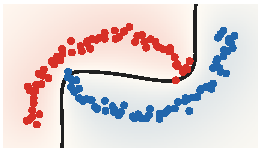
\includegraphics[width=.30\linewidth]{figures/kantorovich-dro-ambiguity/rho-zero.pdf} &
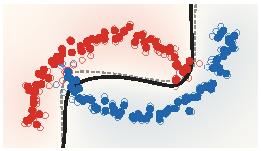
\includegraphics[width=.30\linewidth]{figures/kantorovich-dro-ambiguity/rho-medium.pdf} &
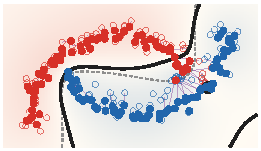
\includegraphics[width=.30\linewidth]{figures/kantorovich-dro-ambiguity/rho-large.pdf} \\[-.15em]
{\small $\rho=0$} &
{\small $\rho=0.055$} &
{\small $\rho=0.11$}
\end{tabular}
\caption{\emph{Wasserstein robustness reshapes the separator between two noisy interlocking moons.} Filled dots are the observed classes, the black curve is the learned zero-score boundary, and the background encodes the logistic probability. The opposing tips of the red and blue crescents overlap locally, forcing the nominal classifier to wind through a narrow nonlinear channel. In the robust panels, the dashed gray curve recalls this nominal boundary; hollow dots show all adversarial locations, while violet segments display a representative half of their transports. As $\rho$ increases, the separator moves away from the most fragile overlap regions and trades clean fit for wider margins. The root-mean-square displacement equals the global quadratic Wasserstein budget $\rho$.}
\label{fig:kantorovich-dro-ambiguity}
\end{figure}

Applied to $c=d^p$, Proposition~\ref{prop-kantorovich-value-curvature} shows that $(\al,\be)\mapsto\Wass_p(\al,\be)^p$ is jointly convex. Thus $\Wass_1$ itself is jointly convex, but $\Wass_p$ need not be convex for $p>1$: on the real line,
\[
	\Wass_p\big((1-t)\delta_0+t\delta_1,\delta_0\big)=t^{1/p},
\]
which is strictly concave for $p>1$.
\index{metric!learning}% strictindex

This convexity is useful when distributions themselves are decision variables. In the usual DRO problem, however, the ambiguity set is fixed once the data are fixed. Therefore, if $z\mapsto\ell_\theta(z)$ is measurable and $\theta\mapsto\ell_\theta(z)$ is convex for every $z$, then
\[
	\theta\mapsto
	\sup_{\be:\,\Wass_p(\be,\widehat{\al}_n)\leq\rho}
	\int \ell_\theta\,\d\be
\]
is convex as a supremum of convex functions of $\theta$. This explains why Wasserstein DRO can preserve convex learning formulations while still modeling adversarial distributional shifts.
\index{convex!function}% strictindex

\paragraph{\texorpdfstring{$\Wass_\infty$}{W-infinity} robustness.}
\index{Wasserstein!infinity distance}% strictindex
\index{Wasserstein!infinity robustness}% strictindex

Worst-case displacement requires an essential-supremum counterpart of the finite-$p$ Wasserstein distances.
\begin{defn}[$\Wass_\infty$ distance]\label{def-wasserstein-infinity}
For probability measures $\al,\be$ on a metric space $(\Xx,d)$, define
\begin{equation}\label{eq-wass-infty}
	\Wass_\infty(\al,\be)
	\eqdef
	\inf_{\pi\in\Couplings(\al,\be)}
	\operatorname*{ess\,sup}_{(x,y)\sim\pi} d(x,y)
\end{equation}
with value $+\infty$ if no finite-displacement coupling exists.
Equivalently,
\[
	\Wass_\infty(\al,\be)\leq r
	\quad\Longleftrightarrow\quad
	\exists\,\pi\in\Couplings(\al,\be)
	\text{ supported on }\{(x,y):d(x,y)\leq r\}.
\]
\end{defn}
This is the limit of $\Wass_p(\al,\be)$ as $p\to\infty$ on bounded spaces, not the limit of the linear objectives defining $\Wass_p^p$. It minimizes the worst displacement rather than an average displacement. Although the essential-supremum objective is not linear, Definition~\ref{def-wasserstein-infinity} shows that each sublevel test is a convex feasibility problem.
Thus $\Wass_\infty$ can be approached by threshold search over support-constrained coupling problems. It remains less convenient than a single linear OT problem, but it is natural in robust formulations where every transported sample must stay within a prescribed perturbation radius.

\begin{prop}[$\Wass_\infty$ robust envelope around an empirical law]\label{prop-wasserstein-infty-dro}
\index{empirical!law}% strictindex
\index{robust!envelope}% strictindex
		Let $(\Zz,d)$ be a Polish metric space. Let $\widehat{\al}=\sum_{i=1}^n a_i\delta_{z_i}$ with distinct $z_i$, positive $a_i$, and $\sum_i a_i=1$, and assume that the closed balls $\overline B(z_i,\rho)$ are compact. Repeated atoms can always be merged to meet this convention. For any real-valued upper-semicontinuous loss $\ell$,
	\[
		\sup_{\be:\,\Wass_\infty(\be,\widehat{\al})\leq\rho}
		\int \ell(z)\d\be(z)
		=
		\sum_{i=1}^n a_i\sup_{z\in\overline B(z_i,\rho)}\ell(z).
	\]
\end{prop}
\begin{proof}
	If $\Wass_\infty(\be,\widehat{\al})\leq\rho$, then, by symmetry, there are couplings $\pi_m\in\Couplings(\widehat{\al},\be)$ whose essential displacements are at most $\rho+1/m$. Since the two marginals are fixed probability measures on a Polish space, $\Couplings(\widehat{\al},\be)$ is tight and closed, hence weakly compact by Prokhorov's theorem. After extraction, $\pi_m\rightharpoonup\pi\in\Couplings(\widehat{\al},\be)$.
\index{probability measure}% strictindex
\index{Prokhorov theorem}% strictindex
\index{Polish space}% strictindex
	For every $\eta>0$, the closed set $F_\eta=\{(x,z):d(x,z)\leq\rho+\eta\}$ has $\pi_m(F_\eta)=1$ for all sufficiently large $m$. Portmanteau's theorem gives $\pi(F_\eta)=1$. Letting $\eta\downarrow0$ along a countable sequence gives $\pi(\{(x,z):d(x,z)\leq\rho\})=1$.
	Disintegrating $\pi$ with respect to the first marginal gives $\pi=\sum_i a_i\delta_{z_i}\otimes\nu_i$, where each $\nu_i$ is supported in the closed ball $\overline B(z_i,\rho)$ and $\be=\sum_i a_i\nu_i$. Hence
	\[
		\int\ell\,\d\be
		=
		\sum_i a_i\int\ell\,\d\nu_i
		\leq
		\sum_i a_i\sup_{\overline B(z_i,\rho)}\ell.
	\]
	The reverse inequality follows by choosing, for each $i$, a maximizer $z_i^\star\in\overline B(z_i,\rho)$ and setting $\be=\sum_i a_i\delta_{z_i^\star}$. The coupling $\sum_i a_i\delta_{(z_i,z_i^\star)}$ has essential displacement at most $\rho$, so this $\be$ is feasible and attains the displayed value.
\end{proof}

The Wasserstein viewpoint developed in this chapter turns transport costs into a geometry with meaningful notions of interpolation, convergence and stability. The next chapter adds the complementary dual description, in which marginal constraints are represented by Kantorovich potentials.
